\documentclass[11pt]{article}

\usepackage{cmap}
\usepackage[T2A]{fontenc}
\usepackage{a4wide}
\usepackage[utf8]{inputenc}
\usepackage[russian]{babel}
\usepackage{vmargin}

\usepackage{graphicx}
\usepackage{subcaption}
\usepackage{float}

\usepackage{color}
\usepackage{indentfirst}

\usepackage{amsmath}
\usepackage{amsthm}
\usepackage{amssymb}
\numberwithin{equation}{section}
%\numberwithin{equation}{subsection}

\setpapersize{A4}
\setmarginsrb{3cm}{2cm}{2cm}{2cm}{0pt}{0mm}{0pt}{13mm}

\theoremstyle{plain}
\newtheorem{thm}{Теорема}[section]
\newtheorem{cor}{Следствие}[section]
\newtheorem{rem}{Замечание}[section]
\newtheorem{problem}{Задача}
\newtheorem{lem}{Утвержение}[section]
\newtheorem{prop}{Свойство}[section]

\theoremstyle{definition}
\newtheorem{defin}{Определение}[section]
\newtheorem{task}{Упражнение}[section]
\newtheorem{exm}{Пример}[section]


\DeclareMathOperator{\expon}{e}
\DeclareMathOperator{\comp}{comp}
\DeclareMathOperator{\rank}{rank}
\DeclareMathOperator{\elip}{\mathcal{E}}
\DeclareMathOperator{\argmin}{argmin}
\DeclareMathOperator{\St}{St}
\DeclareMathOperator{\cl}{cl}


\begin{document}

\setcounter{page}{2}

\tableofcontents
\newpage

\section{Математическая постановка дифференциальной задачи}
В прямоугольной области
\[\Pi = [0,2]\times[0,2]\]
найти дважды гладкую функцию \(u = u(x,y)\) удовлетворяющую уравнению
\begin{equation}
\label{eq}
    -\Delta u = F(x,y), F(x,y) = 2(x^2+y^2)(1-2x^2y^2)\expon^{1-x^2y^2}
\end{equation}
и дополнительному условию
\begin{equation}
\label{BC}
    u(x,y) = \varphi(x,y) = \expon^{1-x^2y^2}
\end{equation}
во всех граничных точках прямоугольника. Оператор Лапласа \(\Delta\) определен равенством:
\[\begin{aligned}
    \Delta u = \frac{\partial^2u}{\partial x^2} + \frac{\partial^2u}{\partial y^2}.
\end{aligned}\]

\section{Численное решение дифференциальной задачи}
Для поиска численного решения задачи~\eqref{eq}-\eqref{BC} используется метод конечных разностей.

В расчётной области \(\Pi\) определим неравномерную прямоугольную сетку
\[\bar w_{h}=\{{(x_i,y_i),\quad i = \overline{0,N_1},\ j=\overline{0,N_2}}\},\]
где
\[\begin{aligned}
x_i = 2f(i/N_1),\quad i = \overline{1,N_1}\\
y_i = 2f(j/N_2),\quad j = \overline{1,N_2}
\end{aligned},\qquad \mbox{здесь }f(t)=\dfrac{(1+t)^{\frac{3}{2}}-1}{2^\frac{3}{2}-1},\quad 0\leqslant t\leqslant 1.
\]
Через \(w_h\) обозначим множество внутренних, а через \(\gamma_h\)~--- множество граничных узлов сетки \(\bar w_{h}.\) Пусть
\[\begin{aligned}
h_i^{(1)} = x_{i+1}-x_{i},\quad i = \overline{1,N_1-1}\\
h_j^{(2)} = y_{i+1}-y_{i},\quad j = \overline{1,N_2-1}
\end{aligned}\]
переменные шаги сетки по оси абсцисс и ординат соответственно. Средние шаги сетки определяются равенствами
\[\begin{aligned}
\bar h_i^{(1)} = \dfrac{h_{i}^{(1)}+h_{i-1}^{(1)}}{2},\quad i = \overline{1,N_1-1}\\
\bar h_j^{(2)} = \dfrac{h_{j}^{(2)}+h_{j-1}^{(2)}}{2},\quad j = \overline{1,N_2-1}
\end{aligned}\]
Рассмотрим линейное пространство \(H\) функций, заданных на сетке \(w_{h}.\) Будем считать, что  пространстве \(H\) задано скалярное произведение и евклидова норма
\[(u,v)=\sum_{i=1}^{N_1-1}\sum_{j=1}^{N_2-1}\bar h_{i}^{(1)}\bar{h}_{j}^{(2)}u(x_{i},y_{i})v(x_i,y_i),\quad\|u\|=\sqrt{(u,u)}.\]
Для аппроксимации уравнения Пуассона~\eqref{eq} воспользуемся пятиточечным разностным оператором Лапласа, который по внутренних узлах сетки определяется равенством:
\[-\Delta_h p_{ij}=\dfrac{1}{\bar{h}_i^{(1)}}\left(\dfrac{p_{ij}-p_{i-1j}}{h_{i-1}^{(1)}}-\dfrac{p_{i+1j}-p_{ij}}{h_{i}^{(1)}}\right)+\dfrac{1}{\bar{h}_{j}^{(2)}}\left(\dfrac{p_{ij}-p_{ij-1}}{h_{j-1}^{(2)}}-\dfrac{p_{ij+1}-p_{ij}}{h_{j}^{(2)}}\right).\]
Здесь предполагается, что функция \(p=p(x_{i},y_{j})\) определена во всех узлах сетки \(\tilde w_{h}.\)
Приближенным решением задачи~\eqref{eq}-\eqref{BC} называется функция \(p=p(x_{i},y_{j}),\) удовлетворяющая уравнениям
\begin{equation}
\label{sheme}
\begin{aligned}
&-\Delta_h p_{ij}=F(x_i,y_j),\quad (x_i,y_j)\in w_{h}\\
&p_{ij}=\varphi(x_{i}y_{i}),\quad (x_{i},y_{j})\in \gamma_{h}.
\end{aligned}
\end{equation}
Эти соотношения представляют собой систему линейных алгебраических уравнений с числом уравнений равным числу неизвестных и определяют единственным образом неизвестные значения \(p_{ij}.\) Совокупность уравнений~\eqref{sheme} называется разностной схемой для задачи~\eqref{eq}-\eqref{BC}.

Приближенное решение системы уравнений~\eqref{sheme} может быть получено итерационным
методом метод скорейшего спуска. В этом методе начальное приближение на границе задается как
\[p_{ij}^{(0)}=\varphi(x_{i},y_{j}),\quad (x_{i},y_{j})\in\gamma_{h},\]
во внутренних узлах сетки \(p_{ij}^{(0)}\) берутся любыми. Метод является одношаговым.
Первая итерация \(p^{(1)}\) вычисляется по формуле
\[p_{ij}^{(1)}=p_{ij}^{(0)}-\tau_{1}r_{ij}^{(0)},\]
где невязка
\begin{equation}
\label{disc}
\begin{aligned}
&r_{ij}^{(k)}=-\Delta_{h}p_{ij}^{(k)}-F(x_i,y_j),\quad (x_{i},y_{j})\in w_{h}\\
&r_{ij}^{(k)}=0,\quad (x_i,y_j)\in\gamma_{h}
\end{aligned}
\end{equation}
а итерационный параметр
\[\tau_{1}=\dfrac{(r^{(0)},r^{(0)})}{(-\Delta_h r^{(0)},r^{(0)})}.\]
Известно, что с увеличением номера итерации \(k\) последовательность сеточных функций \(p^{(k)}\)
сходится к точному решению \(p\) задачи~\eqref{sheme} по норме пространства \(H\), то есть
\[\|p-p^{(k)}\|_{H}\rightarrow 0,\qquad k\rightarrow+\infty. \]
Для последующих итераций используется метод сопряженных градиентов.
Дальнейшие итерации вычисляются по формулам
\[p_{ij}^{(k+1)}=p_{ij}^{(k)}-\tau_{k+1}g_{ij}^{(k)}\quad k=1,2\ldots.\]
Здесь
\[\tau_{k+1}=\dfrac{(r^{(k)},g^{(k)})}{(-\Delta_h g^{(k)},g^{(k)})},\]
вектор
\[\begin{aligned}
&g_{ij}^{k}=r_{ij}^{k}-\alpha_{k}g_{ij}^{(k-1)},\quad k=1,2\ldots,\\
&g_{ij}^{(0)}=r_{ij}^{(0)},
\end{aligned}\]
коэффициент
\[\alpha_{k}=\dfrac{(-\Delta_{h}r^{(k)},g^{k-1})}{(-\Delta_h g^{(k-1)},g^{(k-1)})}\]
Вектор невязки \(r^{(k)}\) вычисляется согласно равенствам~\eqref{disc}. Итерационный процесс останавливается, как только
\[\|p^{(n)}-p^{(n-1)}\|<\varepsilon,\]
где \(\varepsilon\) – заранее выбранное положительное число (в предложенном
варианте задания значение \(\varepsilon=10^{-4}\)).

\section{Постановка задания практикума}
Для задачи~\eqref{eq}-\eqref{BC} требуется найти точное решение и построить
приближённое решение на сетке с числом узлов $N_1 = N_2 = 1000$ и
$N_1 = N_2 = 2000$ и определить погрешность решения по формуле:
\[\begin{aligned}
    \psi=\|u(x,y)-p_{ij}\|.
\end{aligned}\]
Расчеты необходимо проводить на многопроцессорных вычислительных комплексах IBM
Blue Gene/P и <<Ломоносов>>.
Расчеты должны быть проведены для следующего числа процессоров: 128, 256 и 512 на
IBM Plue Gene/P и  8, 16, 32, 64 и 128 на суперкомпьютере <<Ломоносов>>.
Для каждого расчёта определить его
продолжительность и ускорение по сравнению с аналогичным расчётом на одном
вычислительном узле.  При распараллеливании программы необходимо использовать
двумерное разбиение области на подобласти прямоугольной формы, в каждой из
которых отношение $\theta$ количества узлов по ширине и длине должно удовлетворять
неравенствам $\frac{1}{2} \leqslant \theta \leqslant 2$.

На IBM Blue Gene/P также необходимо провести исследование параллельных
характеристик гибридной программы MPI/OpenMP и сравнить полученные результаты с
программой, не используещей директивы OpenMP. Гибридная программа должна
использовать только три процессорных ядра.

\section{Программная реализация}
\subsection{Используемые средства параллелизации}
Для нахождения численного решения поставленной задачи, каждый процессор
производит вычисления на своей области сетки. Для вычисления значений на
границе сетки, необходимо получить от соседних процессоров результаты вычислений
в граничных точках их области, и в свою очередь отправить соседям результаты
своих вычислений. Для обмена массивами данных используются функции
\verb|MPI_Send| и \verb|MPI_Recv|.

При продсчёте скалярного произведения каждый процесс сначала подсчитывает сумму
для своей области, затем с помощью вызова \verb|MPI_Allreduce| с операцией
\verb|MPI_SUM| на каждом процессоре подсчитывается сумма для всей области,
которая используестя в дальнейших вычислениях.

Для подсчёта времени работы программы используется функция \verb|MPI_Wtime|,
перед которой вызывается \verb|MPI_Barrier| для синхронизации процессоров.
В качетсве времени работы программы выбирается максимум по всем процессорам
с помощью вызова \verb|MPI_Reduce| с операцией \verb|MPI_MAX| на нулевом
процессоре. Для подсчёта погрешности сначала на каждом процессоре
подсчитывается скалярное произведение сеточной функции $u(x, x)-p_{ij}$ на
саму себя, после чего все значения суммируются с помощью \verb|MPI_Reduce|
на нулевом процессоре, который вычисляет норму как корень из общего скалярного
произведения.

Возможности технологии OpenMP применяются для распараллеливания циклов.
При вычислении значений векторов используется директива
\verb|#pragma omp parallel for|. Сеточные функции представляются в виде
матрицы, поэтому при вычислении значений в узлах сетки необходимо использовать
вложенный цикл. В версии OpenMP 3.x вложенные циклы можно распараллелить
директивой \verb|#pragma omp parallel for collapse (2)|, однако на Blue Gene P
доступна только версия OpenMP 2.x, поэтому используеются директивы
\begin{verbatim}
    #pragma omp parallel
    #pragma omp for schedule (static) private(j)
\end{verbatim}
где \verb|j|~--- счётчик вложенного цикла.
При подсчёте скалярного произведения используется директива
\verb|#pragma omp for schedule (static) reduction(+:sum)|,
где \verb|sum|~--- переменная, в которой аггрегируется сумма.

\subsection{Распределение задач между процессорами}
Расчётная область разбивается на прямоугольники, каждый из которых будет
обрабатываться одним из процессоров. Сначала выбирается количество
процессоров по вертикали и горизонтали таким образом, чтобы соотношение
количества процессоров не превышало 2:1 и на каждой стороне их количество
было степенью двойки (это возможно, поскольку по условию задачи исходное
количество процессоров также равно степени двойки). Например, 256 процессоров
распределятся поровну (по 16 на каждую сторону), а при 128 процессорах~---
16 по вертикали и 8 по горизонтали.
Описанное распределение реализовано в функции \verb|distribute_procs|.

Процессоры распределяются последовательно согласно рангу от левого верхнего угла
по строкам. На рис.\,\ref{distr_procs} показан пример распределения 8-ми
процессоров.

\begin{figure}[ht]
    \centering
    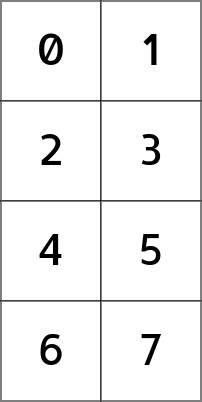
\includegraphics[width=0.2\textwidth]{proc_distr.png}
    \caption{Пример распределения процессоров.}
    \label{distr_procs}
\end{figure}

Далее необходимо определить на каждом процессоре, какие точки сетки будут на
нём обрабатываться. Для каждого процессора определяется сегменты индексов
$[x_1, x_2] \subseteq [0, N_1]$ и $[y_1, y_2] \subseteq [0, N_2]$.
На каждом процессоре сохраняются границы этих интервалов.
Точки распределяются по процессорам поровну, остаток распределяестя по
одной точке на процессор. Таким образом, каждый процессор
обрабатывает
либо $\left \lfloor \frac{N_1}{procs} \right \rfloor + 1$, либо
$\left \lfloor \frac{N_1}{procs} \right \rfloor$ точек по оси $Ox$.
Распределение индексов по оси $Oy$ происходит аналогично.
На рис.\,\ref{distr_points} показан пример распределения вдоль одной из
осей для $procs = 256$, $N = 1000$. Тогда на каждую ось приходится 16 процессоров
и между ними необходимо распределить $N + 1 = 1001$ точку. На первые 9
процессоров приходится 63 точки, на оставшиеся 7~--- 62 точки ($62*7 + 63*9 = 1001$).
Распределение реализовано в функции \verb|distribute_points|.

\begin{figure}[ht]
    \centering
    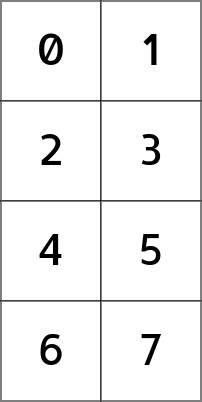
\includegraphics[width=0.2\textwidth]{proc_distr.png}
    \caption{Пример распределения точек по процессорам вдоль одной из осей.}
    \label{distr_points}
\end{figure}

\subsection{Расчёт и обмен данными}

На каждом процессоре после распределения точек происходит инициализация
данных (нулевая итерация), во время которой вычисляются начальные значения
сеточных функций $p$ и $r$. Далее запускается цикл, в котором вычисляется
очередное значение $p$, пока разница между значениями на соседних итерациях
не станет меньше $\varepsilon$. Первая итерация рассчитывается по методу
скорейшего спуска, все последующие~--- методом сопряжённых градиентов.

На каждом процессоре, помимо точек, принадлежащих области, которую обрабатывает
данный процессор, хранятся значение на краницах соседних областей. Эти
значения необходимы при подсчёте оператора Лапласа.
После каждой итерации необходимо обменяться граничными значениями с соседними
процессорами (если они есть). Для избежания взаимных блокировок, обмен
происходит в следующем порядке:
\begin{itemize}
    \item получить строку от верхнего соседа;
    \item получить столбец от левого соседа;
    \item отправить свои значения в порядке вниз, направо, вверх, налево;
    \item получить строку от нижнего соседа;
    \item получить столбец от правого соседа.
\end{itemize}

Таким образом, в начале каждой последующей итерации на каждом процессоре будут
находиться актуальные значения сеточной функции $p$ для обрабатываемой области.
Кроме того, процесоры обмениваются значениями сеточных функций $r$ и $g$ перед
тем, как вычислять оператор Лапласа.

\subsection{Сборка и запуск программы}

Для компиляции программы использовались команды:
\begin{itemize}
    \item Программа с MPI на суперкомпьютере IBM Blue Gene/P:
        \begin{verbatim}
        mpixlcxx_r -O3 main.cpp -o main
        \end{verbatim}
    \item Гибридная программа MPI/OpenMP на суперкомпьютере IBM Blue Gene/P:
        \begin{verbatim}
        mpixlcxx_r -O3 -qsmp=opm main_omp.cpp -o main_omp
        \end{verbatim}
    \item Программа с MPI на суперкомпьютере <<Ломоносов>>:
        \begin{verbatim}
        TODO
        \end{verbatim}
\end{itemize}

Запуск осуществлялся следующим образом:
\begin{itemize}
    \item Программа с MPI на суперкомпьютере IBM Blue Gene/P:
        \begin{verbatim}
        mpisubmit.bg -n PROCS -m smp main -- N1 N2
        \end{verbatim}
    \item Гибридная программа MPI/OpenMP на суперкомпьютере IBM Blue Gene/P:
        \begin{verbatim}
        mpisubmit.bg -n PROCS -m smp -env OMP_NUM_THREADS=3 main_omp -- N1 N2
        \end{verbatim}
    \item Программа с MPI на суперкомпьютере <<Ломоносов>>:
        \begin{verbatim}
        TODO
        \end{verbatim}
\end{itemize}

\newpage
\section{Результаты расчётов}
\begin{table}[h]
\centering
\begin{tabular}{|l|l|l|l|}\hline
Число процессоров $N_p$ & Число точек сетки $N_1 \times N_2$ & Время решения $T$, сек. & Ускорение $S$ \\ \hline
1                       & $1000 \times 1000$                 & 2291.87                 &               \\
2                       & $1000 \times 1000$                 & 1129.8                  & 2.03          \\
128                     & $1000 \times 1000$                 & 21.53                   & 106.45        \\
256                     & $1000 \times 1000$                 & 13.05                   & 175.59        \\
512                     & $1000 \times 1000$                 & 10.3                    & 222.57        \\ \hline
1                       & $2000 \times 2000$                 & ???                     &               \\
2                       & $2000 \times 2000$                 & ???                     &               \\
128                     & $2000 \times 2000$                 & ???                     &               \\
256                     & $2000 \times 2000$                 & ???                     &               \\
512                     & $2000 \times 2000$                 & ???                     &               \\ \hline
\end{tabular}
    \caption{Результаты работы программы (MPI) на IBM Blue Gene/P.}
\label{tab_mpi}
\end{table}

\begin{table}[h]
\centering
\begin{tabular}{|l|l|l|l|}\hline
Число процессоров $N_p$ & Число точек сетки $N_1 \times N_2$ & Время решения $T$, сек. & Ускорение $S$ \\ \hline
1                       & $1000 \times 1000$                 & ???                     & ???           \\
128                     & $1000 \times 1000$                 & ???                     & ???           \\
256                     & $1000 \times 1000$                 & ???                     & ???           \\
512                     & $1000 \times 1000$                 & ???                     & ???           \\ \hline
1                       & $2000 \times 2000$                 & ???                     & ???           \\
128                     & $2000 \times 2000$                 & ???                     & ???           \\
256                     & $2000 \times 2000$                 & ???                     & ???           \\
512                     & $2000 \times 2000$                 & ???                     & ???           \\ \hline
\end{tabular}
    \caption{Результаты работы программы (MPI/OpenMP) на IBM Blue Gene/P.}
\label{tab_mpi}
\end{table}

\begin{table}[h]
\centering
\begin{tabular}{|l|l|l|l|}\hline
Число процессоров $N_p$ & Число точек сетки $N_1 \times N_2$ & Время решения $T$, сек. & Ускорение $S$ \\ \hline
1                       & $1000 \times 1000$                 & ???                     & ???           \\
2                       & $1000 \times 1000$                 & ???                     & ???           \\
8                       & $1000 \times 1000$                 & ???                     & ???           \\
16                      & $1000 \times 1000$                 & ???                     & ???           \\
32                      & $1000 \times 1000$                 & ???                     & ???           \\
128                     & $1000 \times 1000$                 & ???                     & ???           \\ \hline
1                       & $2000 \times 2000$                 & ???                     & ???           \\
2                       & $2000 \times 2000$                 & ???                     & ???           \\
8                       & $2000 \times 2000$                 & ???                     & ???           \\
16                      & $2000 \times 2000$                 & ???                     & ???           \\
32                      & $2000 \times 2000$                 & ???                     & ???           \\
128                     & $2000 \times 2000$                 & ???                     & ???           \\ \hline
\end{tabular}
    \caption{Результаты работы программы на СК <<Ломоносов>>.}
\label{tab_mpi}
\end{table}

\section{Сравнение численного решения с аналитическим}
Функция \[u(x,y)=\expon^{1-x^2y^2}\]
является точным решением задачи~\eqref{eq}-\eqref{BC} в прямоугольнике \(\Pi.\)

\end{document}

